\chapter{Team-klassen}
\begin{minipage}[t]{1\linewidth}
%Set imagepath and scaling, imagepath set to start in images/UmlMini folder, just write filename and extension
%FBox added for outline on items
\begin{wrapfigure}{l}{0.5\textwidth}
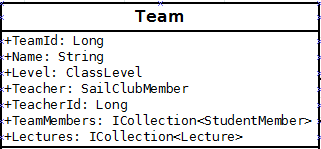
\includegraphics[scale=0.7]{Team_UML.png}
\end{wrapfigure}

Programmet indeholder også en båd klasse. Dataene indeholdt i denne klasser giver sig selv ud fra UML-diagrammet. Der er
også en overordnet klasse for sejlture, som er abstrakt. Denne arver klasserne skoletur og almindelig tur fra. Der skal
for hver sejltur, registreres hvilken båd der bliver brugt samt tidspunkt for afgang og ankomst. Vejrforholdene skal
registres og der kan tilføjes de kommentarer der muligvis kan være. Når der er tale om en almindelig tur, registreres
der hvem kaptajnen er og de øvrige besætningsmedlemmer bliver tilføjet til en liste. Der skal desuden registreres,
hvornår man regner med at være tilbage fra turen, hvad formålet med turen er og hvor man sejler henne. Dette skal
gøres, så det er lettere at finde båden og besætningen, f.eks. i tilfælde af at en ulykke forekommer.
Ved en skoletur er der registret et skolehold, som er defineret i en klasse. Skoleholds klassen indeholder lærer og
elever. Man kan tilføje yderligere elever til en skoletur, som normalt ikke er med, samt gæster som ikke er elever. Der
registreres også hvem der deltager på turen, da der kan være elever fra det normale hold, som ikke møder op. Til
sejlturene er der tilknyttet en skadesrapport, som skal, som navnet angiver, bruges til at registrere hvis der kommer
skader på båden under sejladsen. 

\end{minipage}